\subsection{Emergency Converging}\label{s:testEmergencyConverging}

\paragraph{Scenario:} Two \emph{UAS} are flying in an \emph{uncontrolled airspace} (altitude $\le$ 500 ft. Above the Ground Level) with missions defined in (tab. \ref{tab:missionSetupEmergencyConvergingScenario}). Both \emph{UAS} are in the \emph{Navigation mode} with active \emph{ADSB-In/Out}, receiving position notification from each other. Cruising altitude is sufficient for horizontal separation (50-100 ft. Above the Ground Level). \emph{Horizontal separation} is preferred separation type for both \emph{UAS}.

\begin{table}[H]
    \centering
    \begin{tabular}{c||c|c||c}
        \multirow{2}{*}{UAS} &\multicolumn{2}{c||}{Position} & \multirow{2}{*}{$\mathscr{WP}_1$} \\\cline{2-3}
          & $[x,y,z]$           & $[\theta,\varpi,\psi]$           & \\\hline\hline
        1 & $[0,20,0]^T $       & $[0^\circ,0^\circ,0^\circ]^T$    & $[40,20,0]^T$\\\hline 
        2 & $[20,0,0]^T $       & $[0^\circ,0^\circ,90^\circ]^T$  & $[20,40,0]^T$\\ 
    \end{tabular}
    \caption{Mission setup for \emph{Emergency converging} scenario.}
    \label{tab:missionSetupEmergencyConvergingScenario}
\end{table}

\begin{note}
\emph{Collision point} is expected at $\mathscr{C} = [20,20,0]^T$. The \emph{angle of approach} is $90^{\circ}$ which classifies situation as \emph{Converging maneuver} (fig. \ref{fig:OvertakeManeuverTheoretical}).
\end{note}

\paragraph{Main Goal:} Show two \emph{non-cooperative} UAS avoidance capability for \emph{Converging maneuver} scenario in \emph{uncontrolled airspace}.


\paragraph{Acceptance criteria:}
\begin{enumerate}
    \item \emph{Proper mode invocation} - when an intruder intersects the UAS  with \emph{Right of the Way} navigation grid, both UAS will swith into \emph{Emergency Avoidance Mode}.
    
    \item \emph{Minimal safety margin distance} $\ge$ $0 m$.
    
    \item \emph{Each UAS} will reach own goal waypoint (tab. \ref{tab:missionSetupEmergencyConvergingScenario}).
\end{enumerate}

\paragraph{Testing setup:} The \emph{standard test setup} for each UAS defined in (tab \ref{tab:testMovementOrientations}, \ref{tab:testUASBasicParameters}, \ref{tab:testNavigationGridBasic}, \ref{tab:testAvoidanceGridBasic}, \ref{tab:testUASColoring}) is used with following without parameter override.

\emph{Intruder intersection} model has been chosen depending on UAS (tab. \ref{tab:aboidanceParametersForEmergencyConvergingScenario}). Each UAS is equipped with \emph{ADS-B In/Out} sensor obtaining/distributing following information:
\begin{enumerate}
    \item \emph{Position} - in operational section coordinate frame.
    \item \emph{Velocity} - vector representation in given coordinate frame.
    \item \emph{Class size} - class body radius based on UAS propulsion and size.
    \item \emph{Safety margin set} - set of safety margins for different collision cases.
\end{enumerate}

\noindent \emph{Avoidance parameters} for \emph{Emergency converging scenario} are given in (tab. \ref{tab:aboidanceParametersForEmergencyConvergingScenario}). Each UAS has same speed set to $1 m s^{-1}$. Second UAS has the \emph{Right of The Way}. 

\emph{Safety margin} is considered as sum of both participants \emph{near miss margins}. In this case default safety margin is considered as $1.2$ $m$.

\begin{table}[H]
    \centering
    \begin{tabular}{c||c|c|c||c|c||c}
        \multirow{2}{*}{UAS} & \multicolumn{3}{c||}{Parameters} & \multicolumn{2}{c||}{Margins} & \multirow{2}{*}{Separation}                                            \\\cline{2-6}
                             & velocity & intruder model & ROW        & body & safety \\\hline\hline
        1                    & 1        & body + spread  & false            & 0.3         & 0.6           & horizontal\\\hline
        2                    & 1        & body + spread  & true             & 0.3         & 0.6  & horizontal          \\
    \end{tabular}
    \caption{Avoidance parameters for  \emph{Emergency converging} scenario.}
    \label{tab:aboidanceParametersForEmergencyConvergingScenario}
\end{table}

\begin{note}
 Both UAS are using  body (sec. \ref{s:bodyvolumeIntersection}) and spread (sec \ref{s:uncertaintyIntersection}) intersection models, reflecting both body volume and maneuverability  of intruder. Both UAS have preferred separation mode as \emph{horizontal}, typical for planes.
\end{note}

\paragraph{Simulation Run:} Notable moments from the simulation run (fig. \ref{fig:testCaseEmergencyConverging}) are following
\begin{enumerate}
    \item \emph{Detection} (fig. \ref{fig:emergencyConvergingSituationDetection}) - Intruder (UAS2 cyan) is approaching (UAS 1 blue) from right side, Intruder (UAS2 cyan) has the right of the way, because $70^{\circ}$ $\le$ $angleOfApproach$ $<$ $130^{\circ}$. \emph{Intruder intersection model} (for UAS 2) is created and propagated in \emph{avoidance grid} (for UAS 1). 
            
    \item \emph{Start Converging} (fig. \ref{fig:emergencyConvergingStart}) - when \emph{UAS 2 (cyan) parametric intruder intersection model} disables \emph{trajectories}, converging maneuver for UAS 1 (blue) starts.
    
    \item \emph{Near miss case} (fig. \ref{fig:emergencyConvergingEnd}) - UAS 1 (blue) to UAS 2 (cyan) closest distance. The safety margin for \emph{near miss} has not been breached. The safety margin for \emph{well clear} in uncontrolled airspace is invalid.
    
    \item \emph{Waypoint reached} (fig. \ref{fig:emergencyConvergingWaypointReach}) - the intruder intersection model for \emph{UAS 2} (cyan) is removed from UAS 1 (blue) \emph{avoidance grid} after \emph{converging maneuver competition}, standard navigation procedure is applied afterwards.
    
    \item Note that \emph{UAS 2} (cyan) has \emph{Right of the way} in (tab. \ref{tab:aboidanceParametersForEmergencyConvergingScenario}).
    
    \item Note that \emph{UAS 1} (blue) used only horizontal separation (priority) in (fig. \ref{fig:emergencyConvergingUAS1PathTracking}).
\end{enumerate}


\begin{figure}[H]
    \centering
    \begin{subfigure}{0.48\textwidth}
    	\centering
        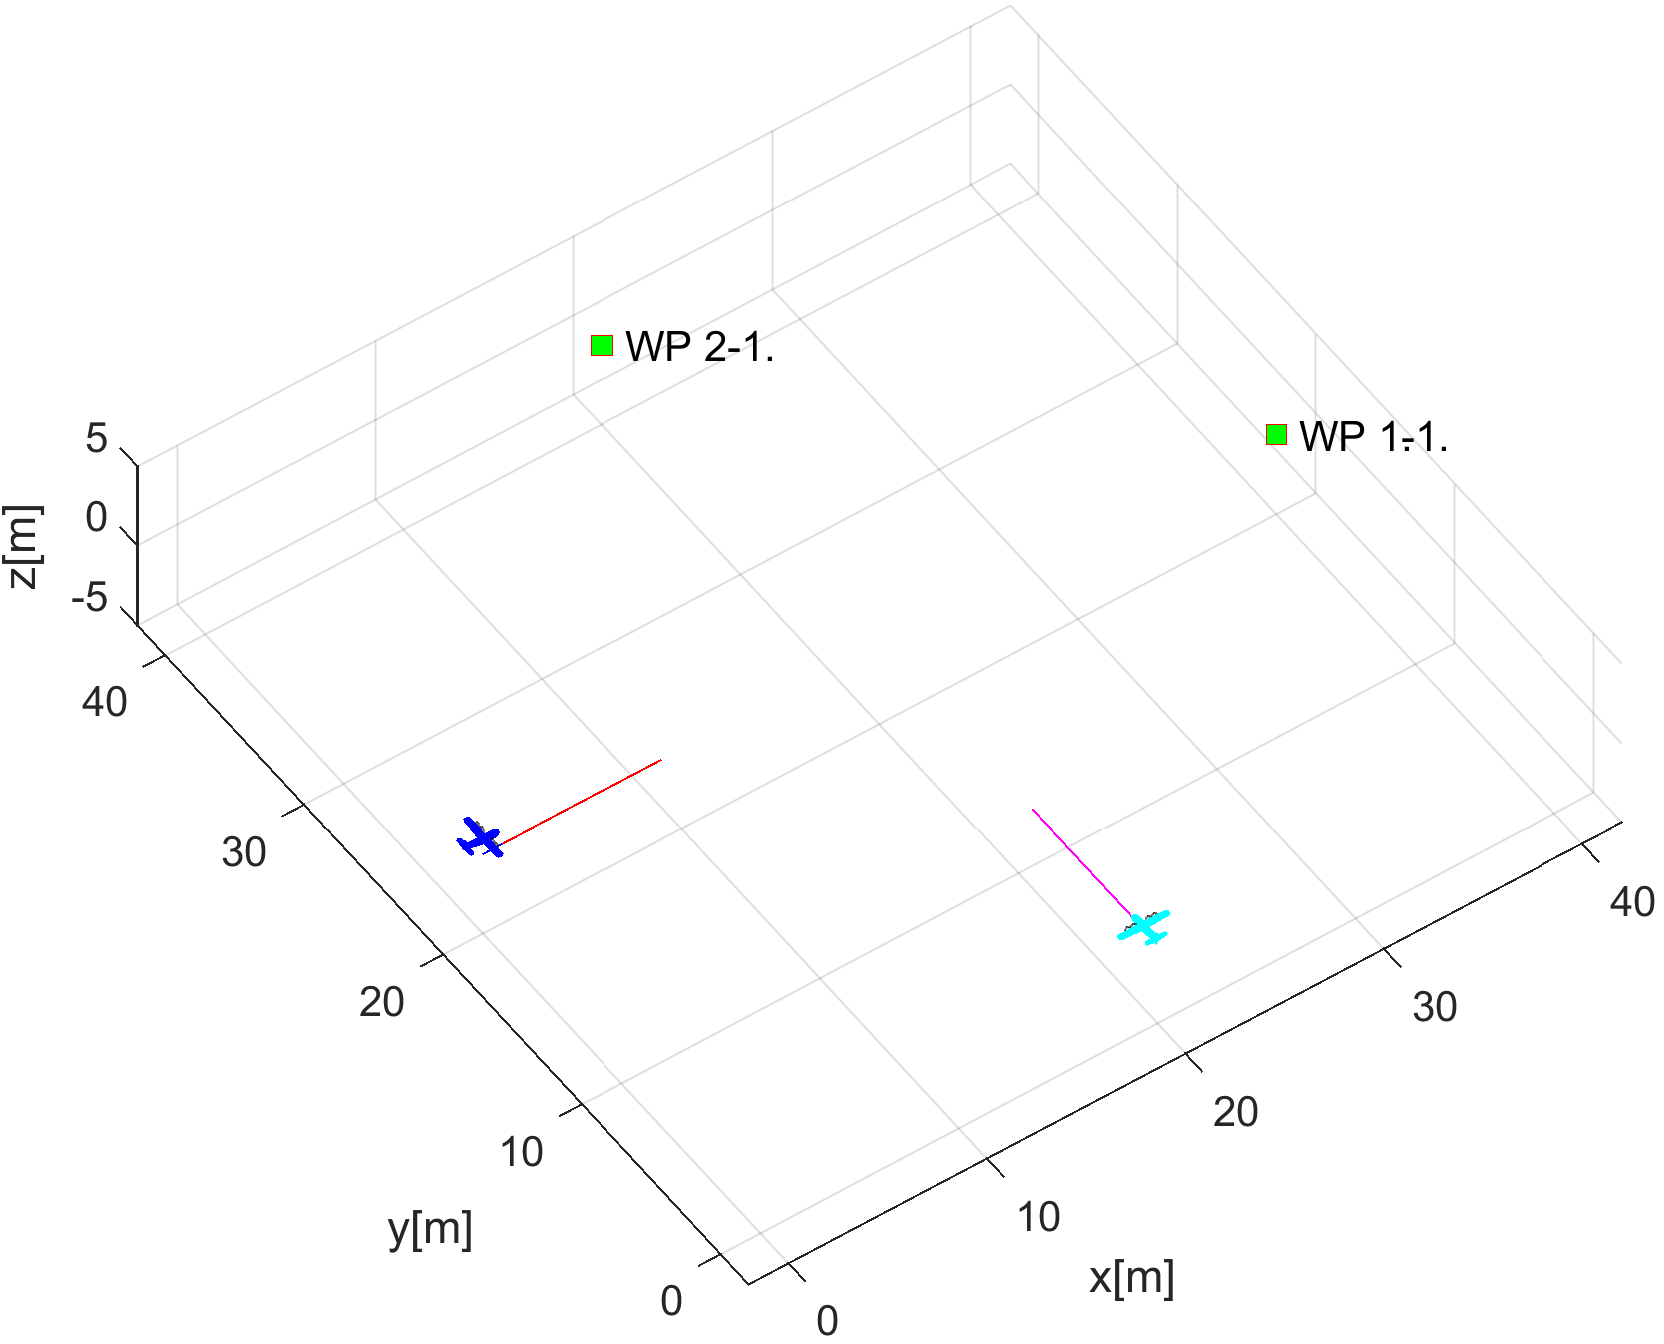
\includegraphics[width=0.9\linewidth]{\FIGDIR/NS025UtmEmergencyConverging00001}
        \caption{Situation detection.}
        \label{fig:emergencyConvergingSituationDetection}
    \end{subfigure}
    \begin{subfigure}{0.48\textwidth}
    	\centering
        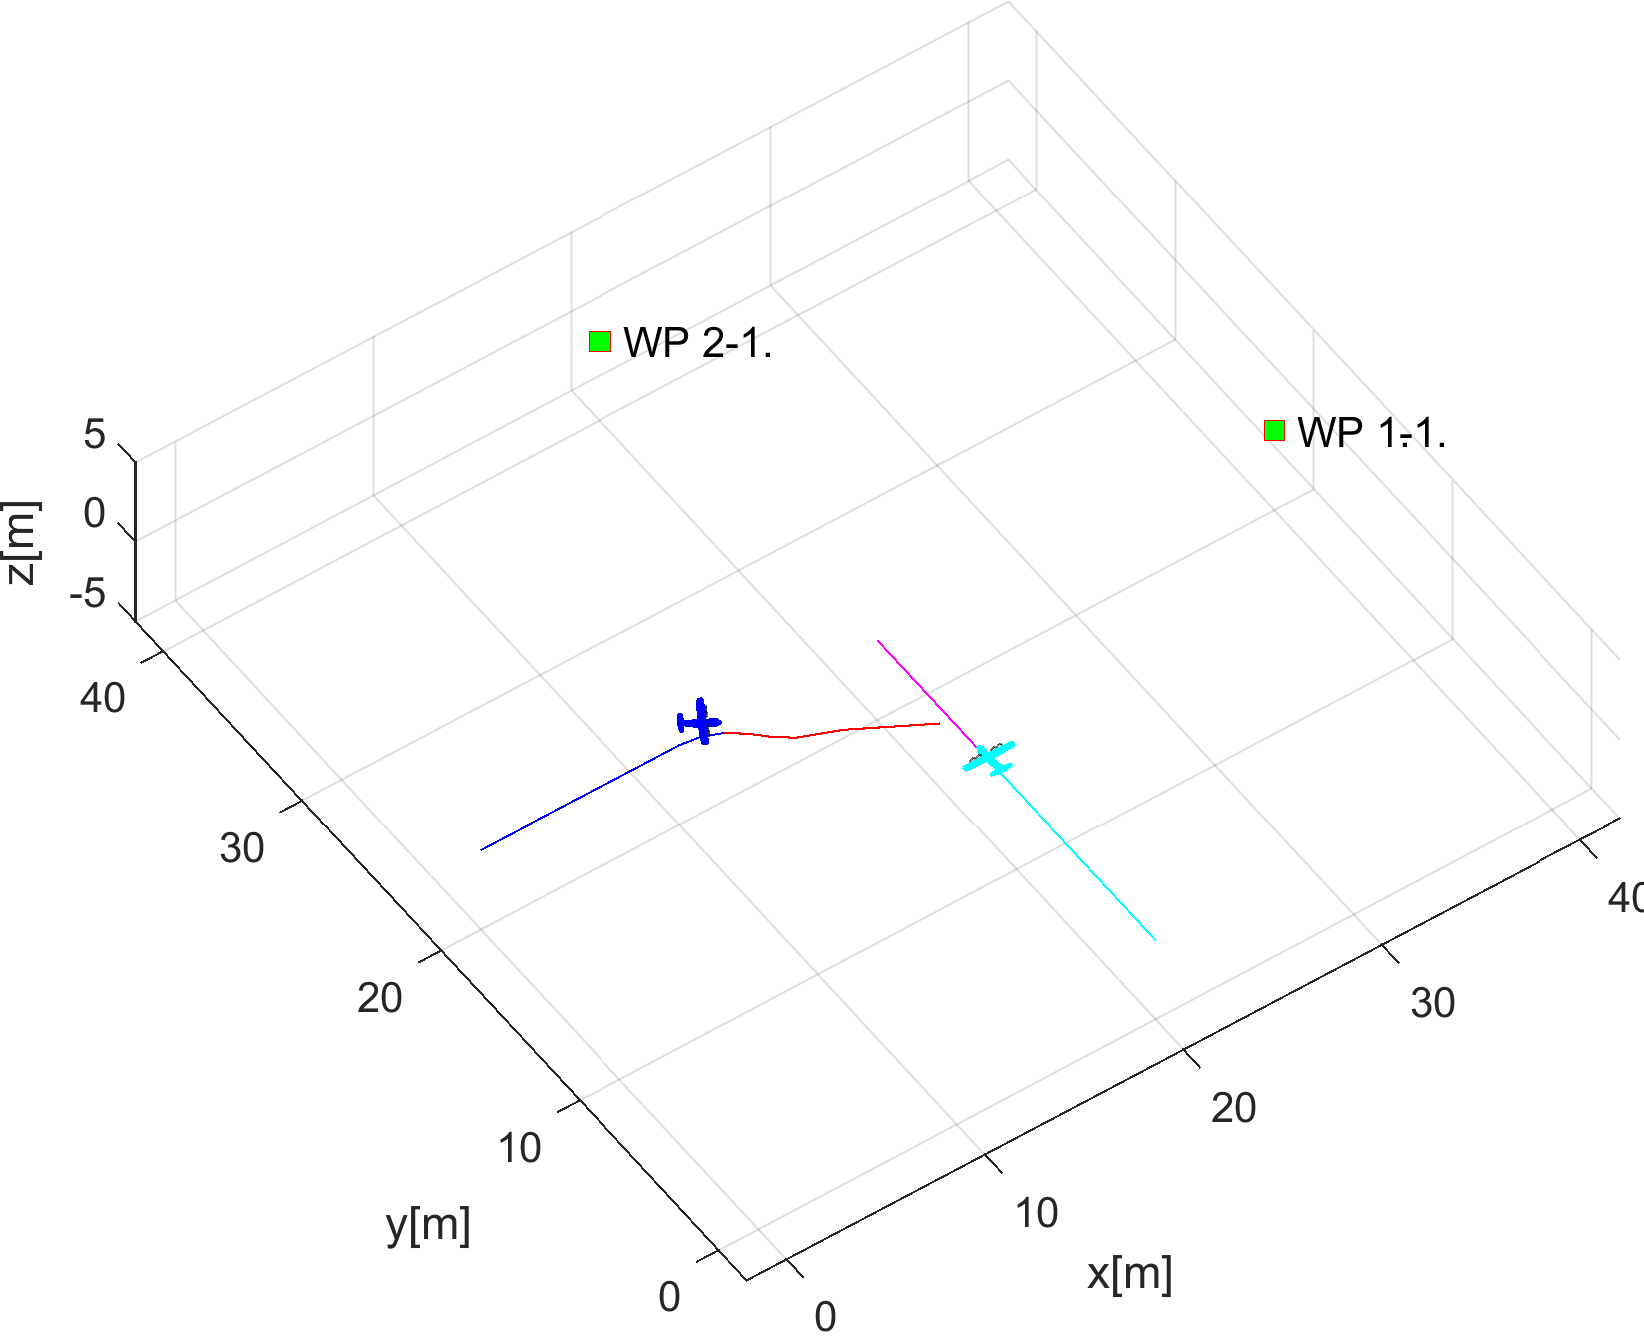
\includegraphics[width=0.9\linewidth]{\FIGDIR/NS026UtmEmergencyConverging00012} 
        \caption{Start converging.}
        \label{fig:emergencyConvergingStart}
    \end{subfigure}
    \\
    \begin{subfigure}{0.48\textwidth}
    	\centering
        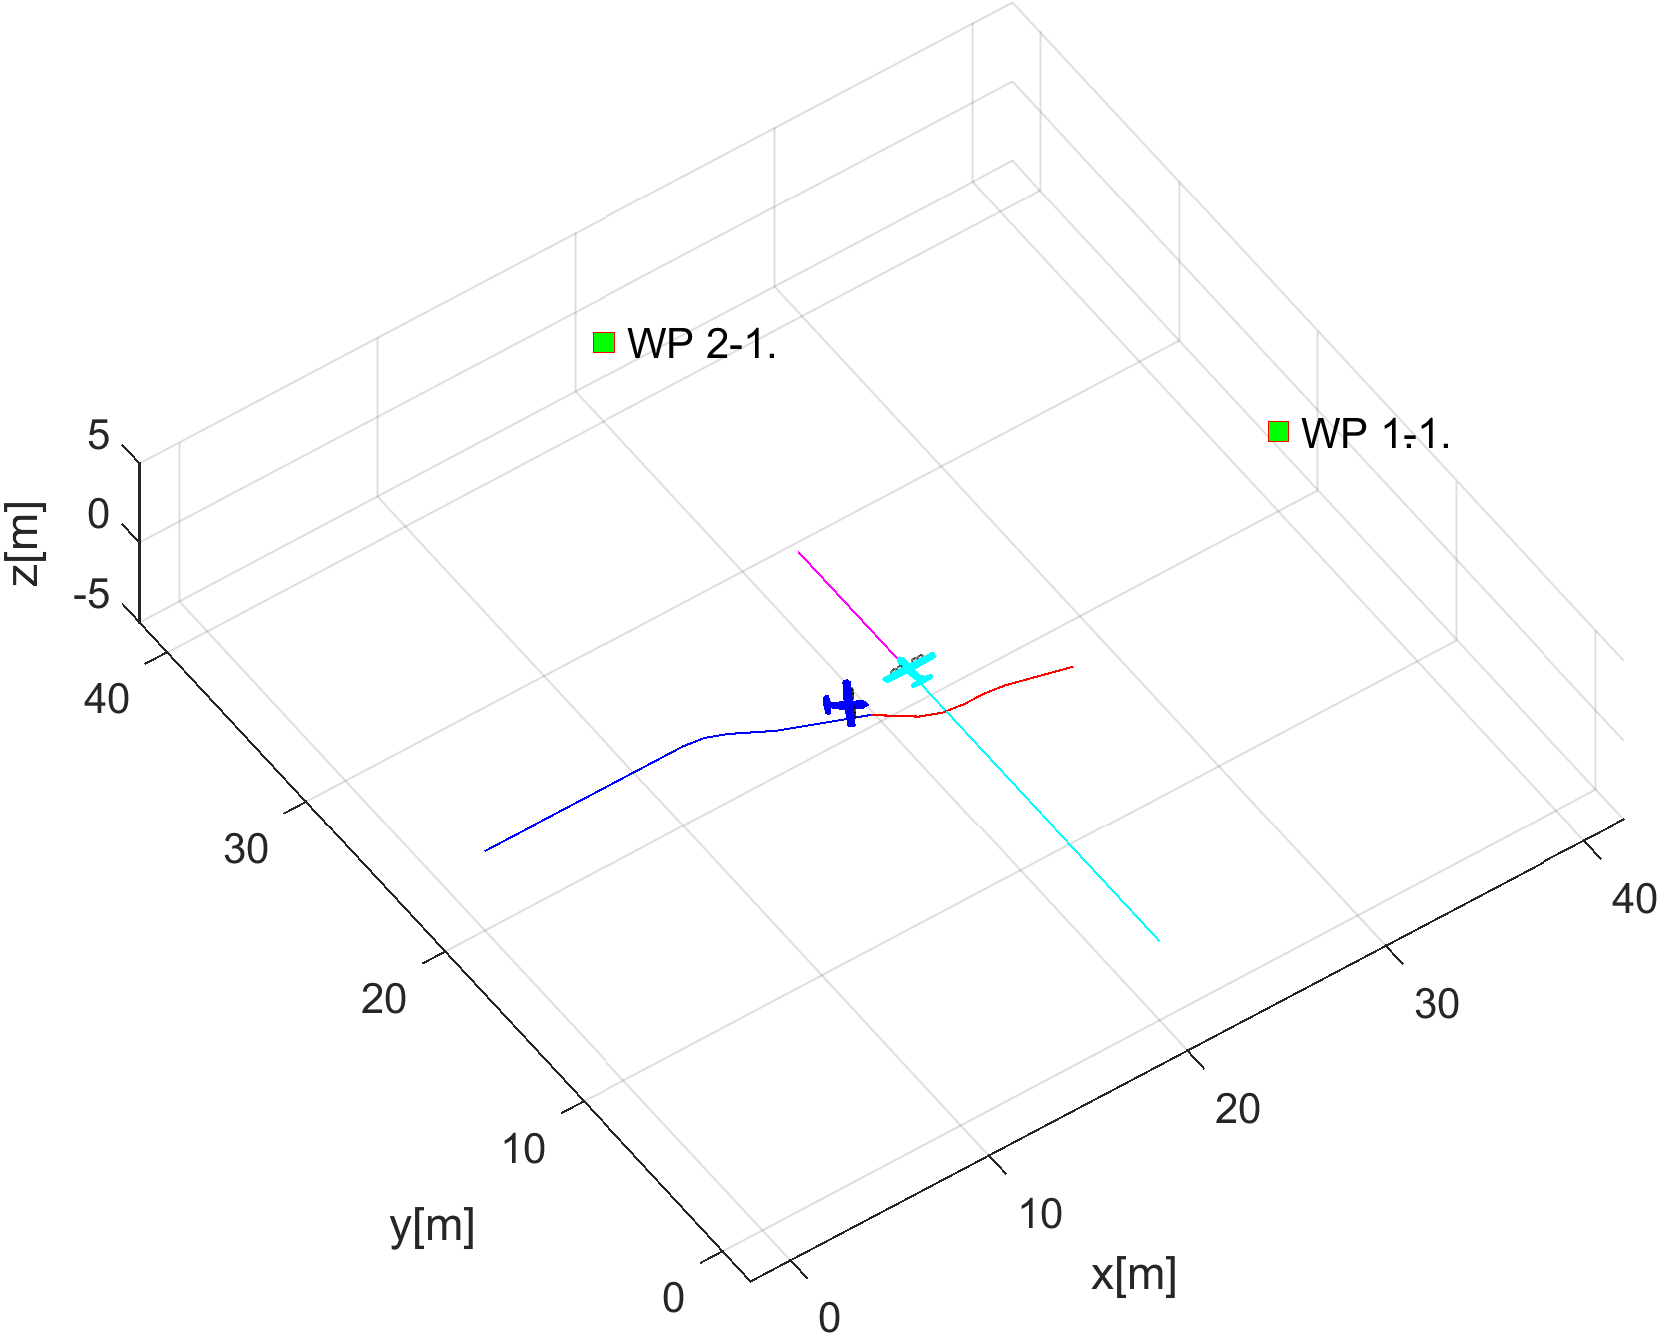
\includegraphics[width=0.9\linewidth]{\FIGDIR/NS027UtmEmergencyConverging00018} 
        \caption{Near miss case.}
        \label{fig:emergencyConvergingEnd}
    \end{subfigure}
    \begin{subfigure}{0.48\textwidth}
    	\centering
        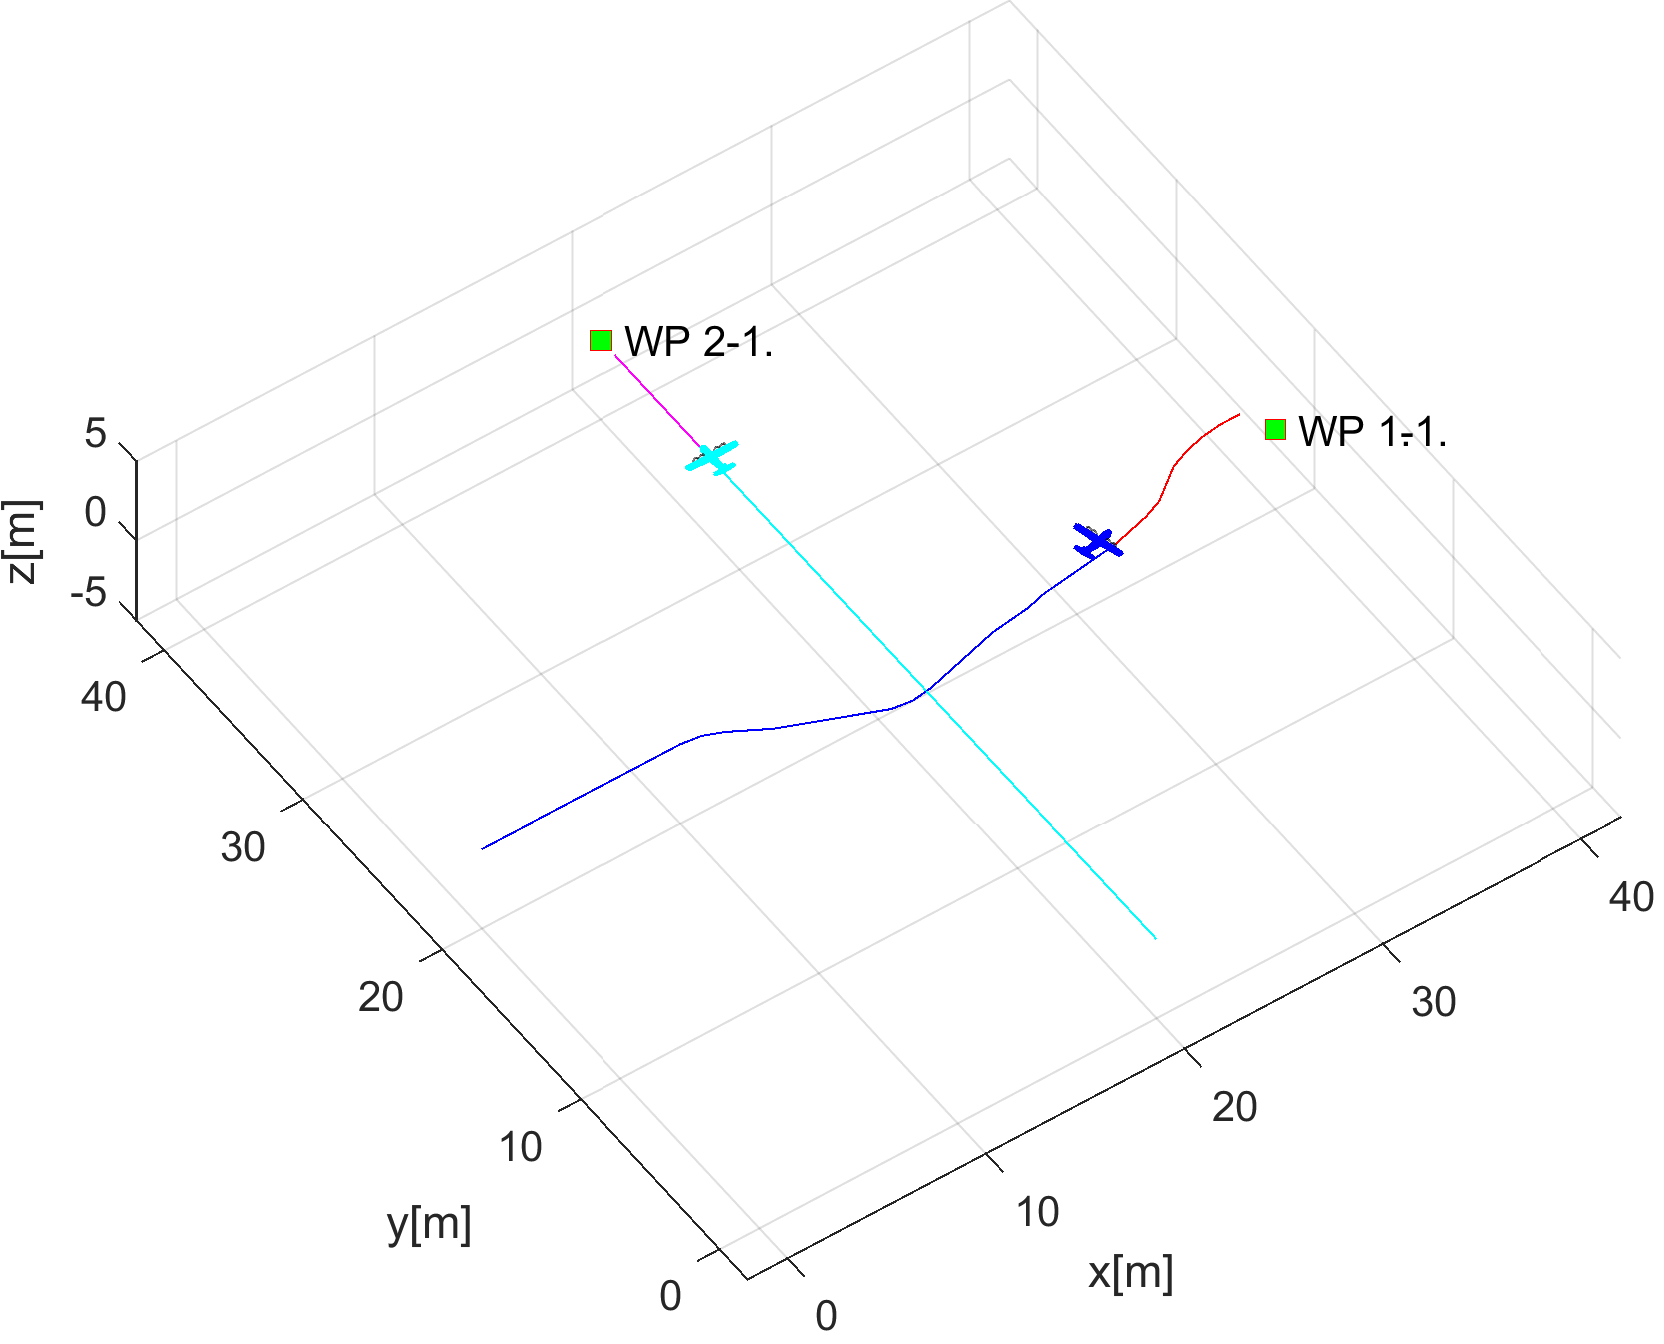
\includegraphics[width=0.9\linewidth]{\FIGDIR/NS028UtmEmergencyConverging00032} 
        \caption{Waypoints reach.}
        \label{fig:emergencyConvergingWaypointReach}
    \end{subfigure}
    \caption{Test scenario for \emph{Emergency converging} (Intruder avoidance). }
    \label{fig:testCaseEmergencyConverging}
\end{figure}


\paragraph{Safety Margin Performance:} There is need to compare mutual distance between both UAS (y-axis [m]) and its evolution over UTM time (x-axis [s]). The \emph{mutual} distance of \emph{UAS 1} to \emph{UAS 2} is given by \emph{blue line}. The \emph{Safety margin} value is denoted by red line at \emph{constant value} of $1.2m$.

The \emph{Proper avoidance Invocation} is shown when UAS systems are getting closer to each other and they start their separation phase (Emergency Avoidance Mode). The \emph{Mutual distance} (blue line) does not cross \emph{safety margin} (red line).

\begin{figure}[H]
    \centering
    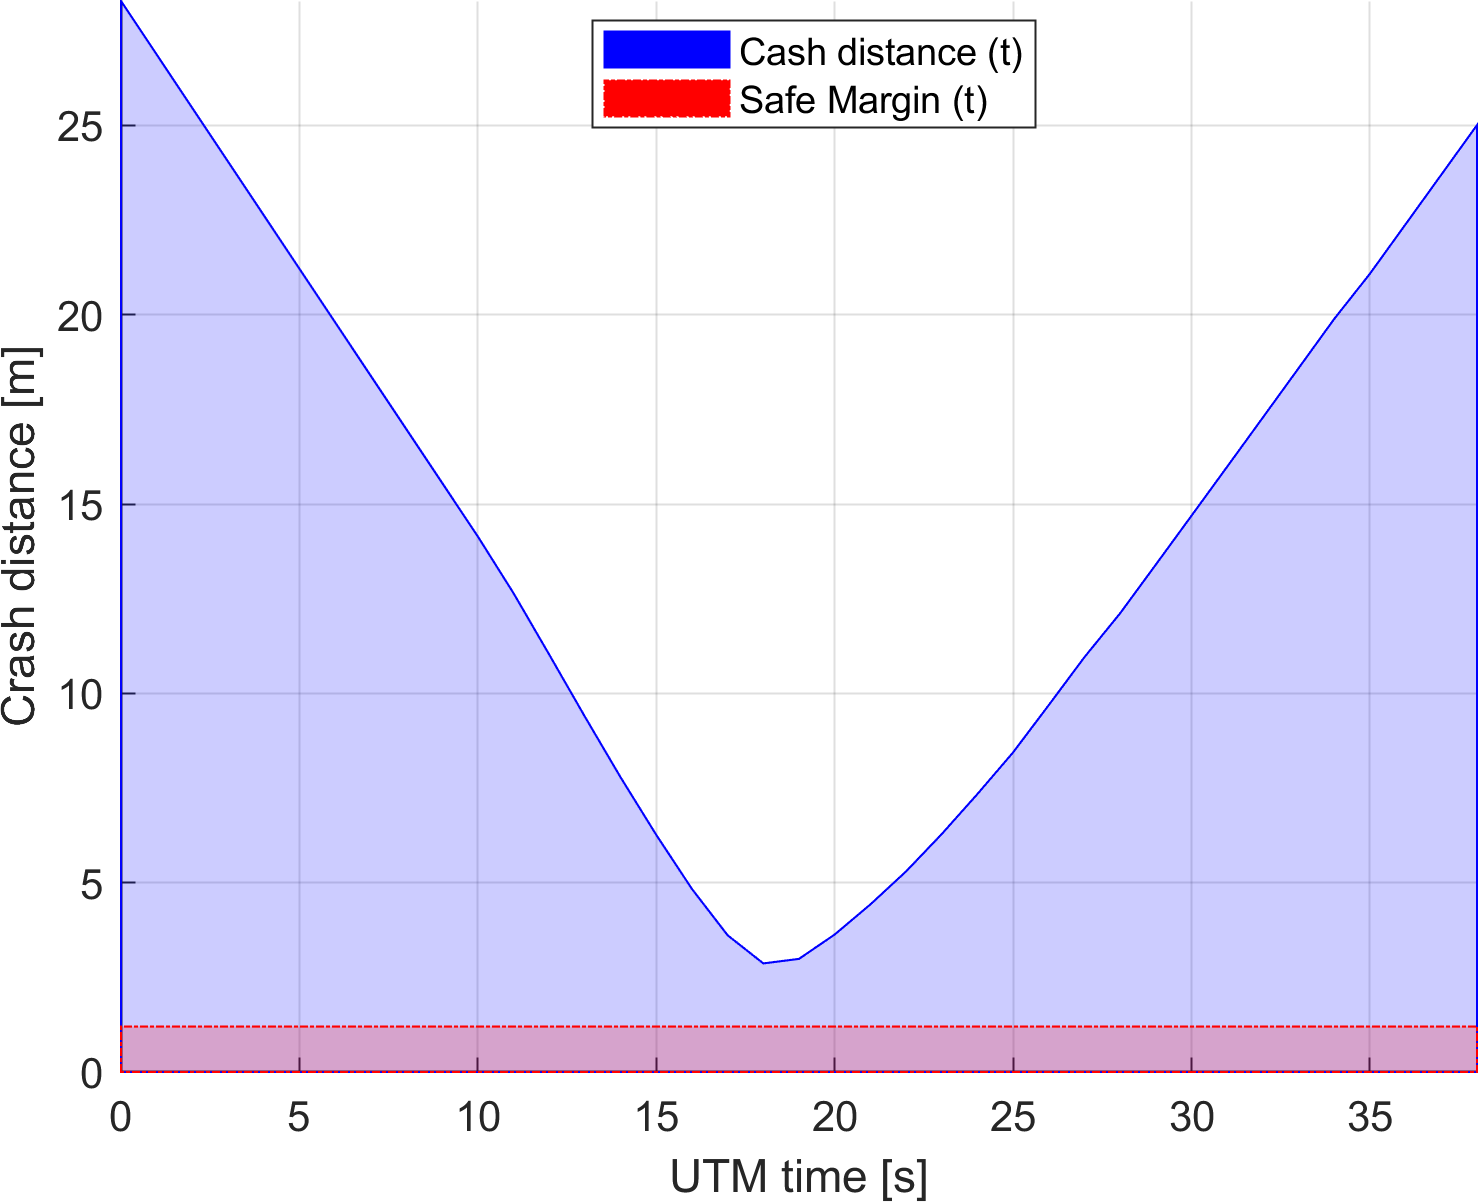
\includegraphics[width=0.55\linewidth]{\FIGDIR/NS029UtmEmergencyConvergingPerformance} 
    \caption{\emph{Emergency converging} safety margin performance.}
    \label{fig:testCaseEmergencyConvergingAvoidancePerformance}
\end{figure}

\paragraph{Safety Margin Distance:} Minimal and Maximal mutual distance to safety margi is summarized in (tab. \ref{tab:testCaseEmergencyConvergingSafetyMarginDistances}). The closest to collision are UAS systems when distance to safety margin is $1.6676m$.

The \emph{minimal safety margin distance $\ge$ 0} which means that the \emph{safety acceptance criterion} is full filled. 

\begin{table}[H]
    \centering
    \begin{tabular}{c|c||c}
    \multicolumn{2}{c||}{UAS:} & 1-2 \\\hline\hline
    \multirow{2}{*}{safety margin distance} & min & 1.6676 \\\cline{2-3}
                                            & max & 27.0843 \\
    \end{tabular}
    \caption{\emph{Emergency converging} safety margin distances.}
    \label{tab:testCaseEmergencyConvergingSafetyMarginDistances}
\end{table}

\paragraph{Path Tracking Performance:} All waypoints (green numbered squares) for both  UAS have been reached (fig. \ref{fig:emergencyConvergingTrajectoryTrackingPerformance}). \emph{Reference trajectories} (green dashed lines), between initial position (green square marked S) and goal waypoint (green square marked 1) are split into three XYZ values with respective figures. The tracked value is on y-axis [m] and time on x-axis [s]. The blue lines represents real parameter evolution over time.

Following observations can be made from path tracking (fig. \ref{fig:emergencyConvergingTrajectoryTrackingPerformance}) and preferred separations (tab. \ref{tab:aboidanceParametersForEmergencyConvergingScenario}):

\begin{enumerate}
    \item UAS 1 (fig. \ref{fig:emergencyConvergingUAS1PathTracking}) is using \emph{horizontal separation} (y-axis). The UAS diverges from reference trajectory to minimal necessary time.
    \item UAS 2 (fig. \ref{fig:emergencyCovnergingUAS2PathTracking}) has the right of the way and is not using any active avoidance mechanism. 
\end{enumerate}

\begin{figure}[H]
    \centering
    \begin{subfigure}{0.48\textwidth}
    	\centering
        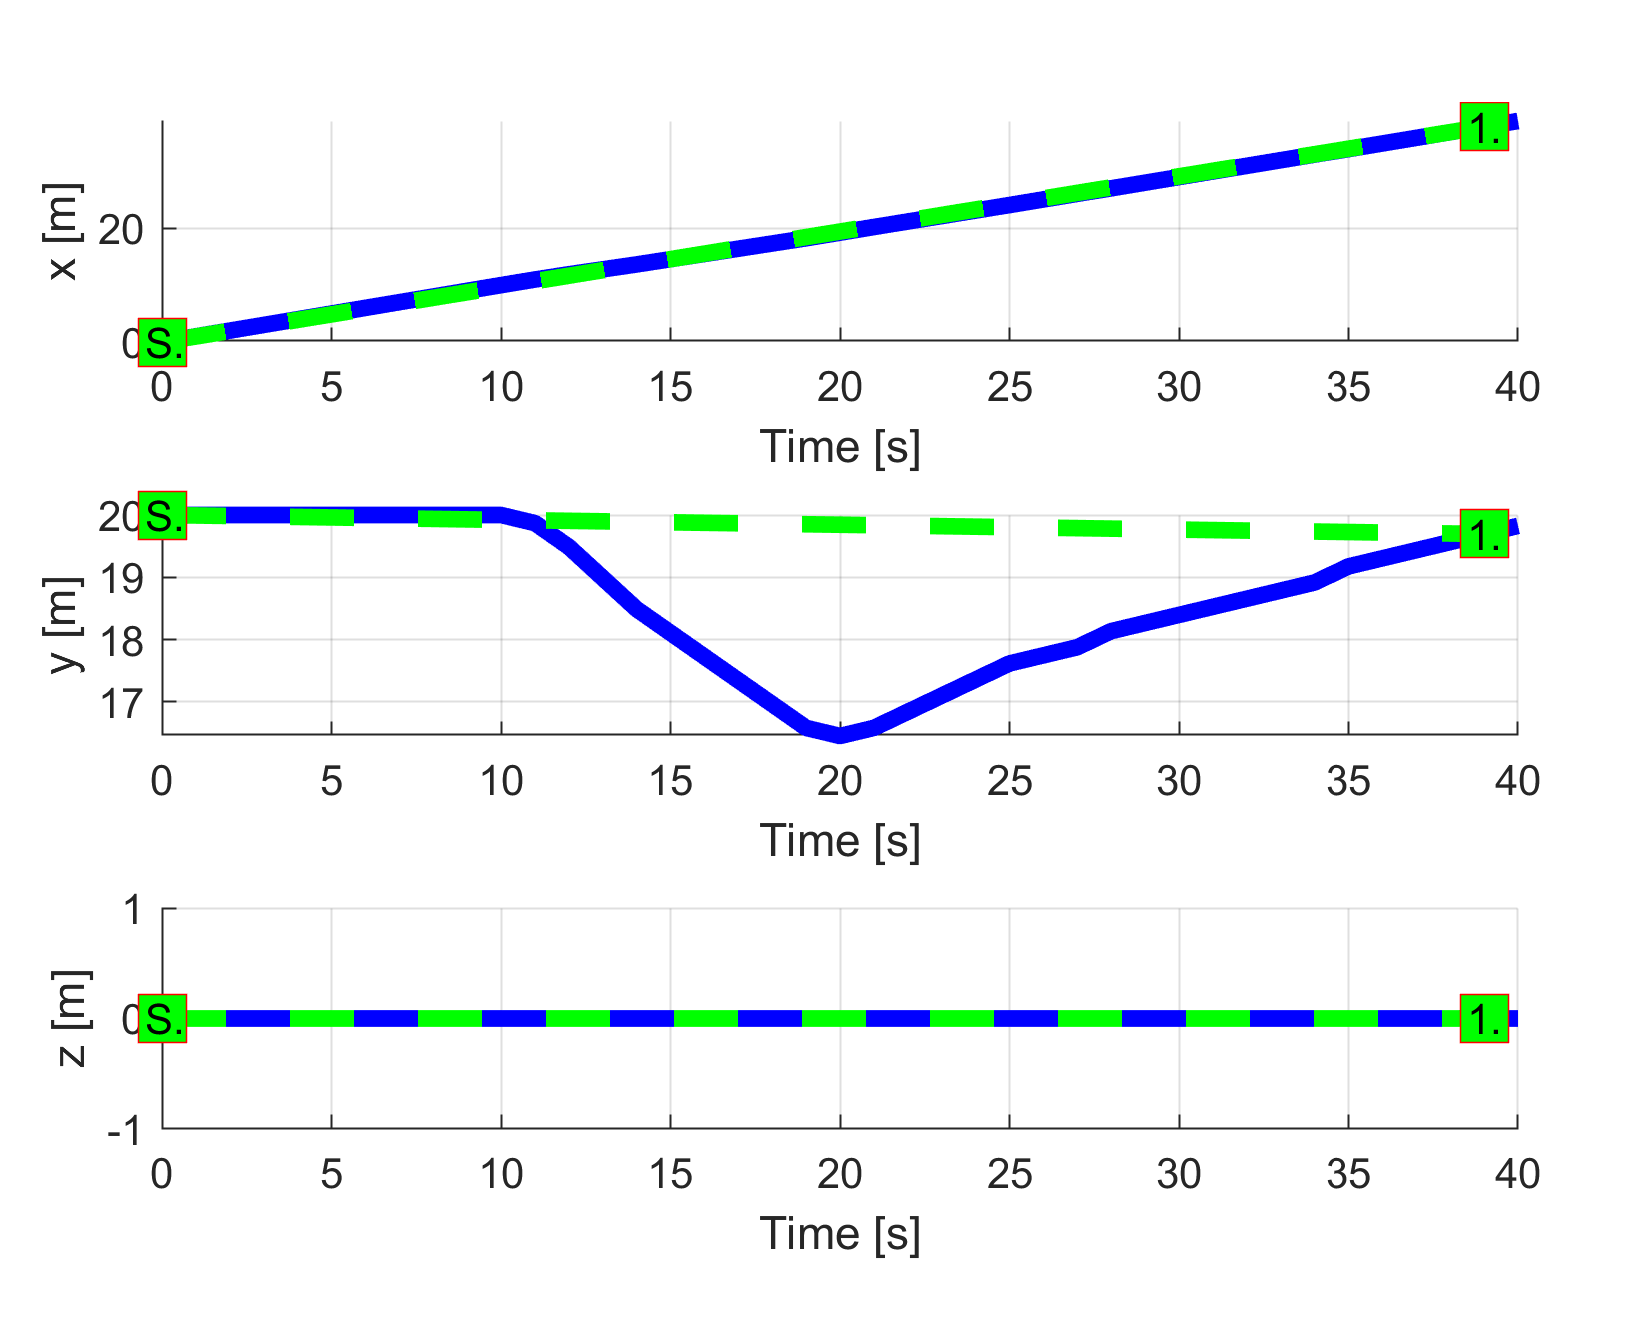
\includegraphics[width=0.9\linewidth]{\FIGDIR/NS030UtmEmergencyConvergingUAV1PathFollowing}
        \caption{UAS 1.}
        \label{fig:emergencyConvergingUAS1PathTracking}
    \end{subfigure}
    \begin{subfigure}{0.48\textwidth}
	    \centering
        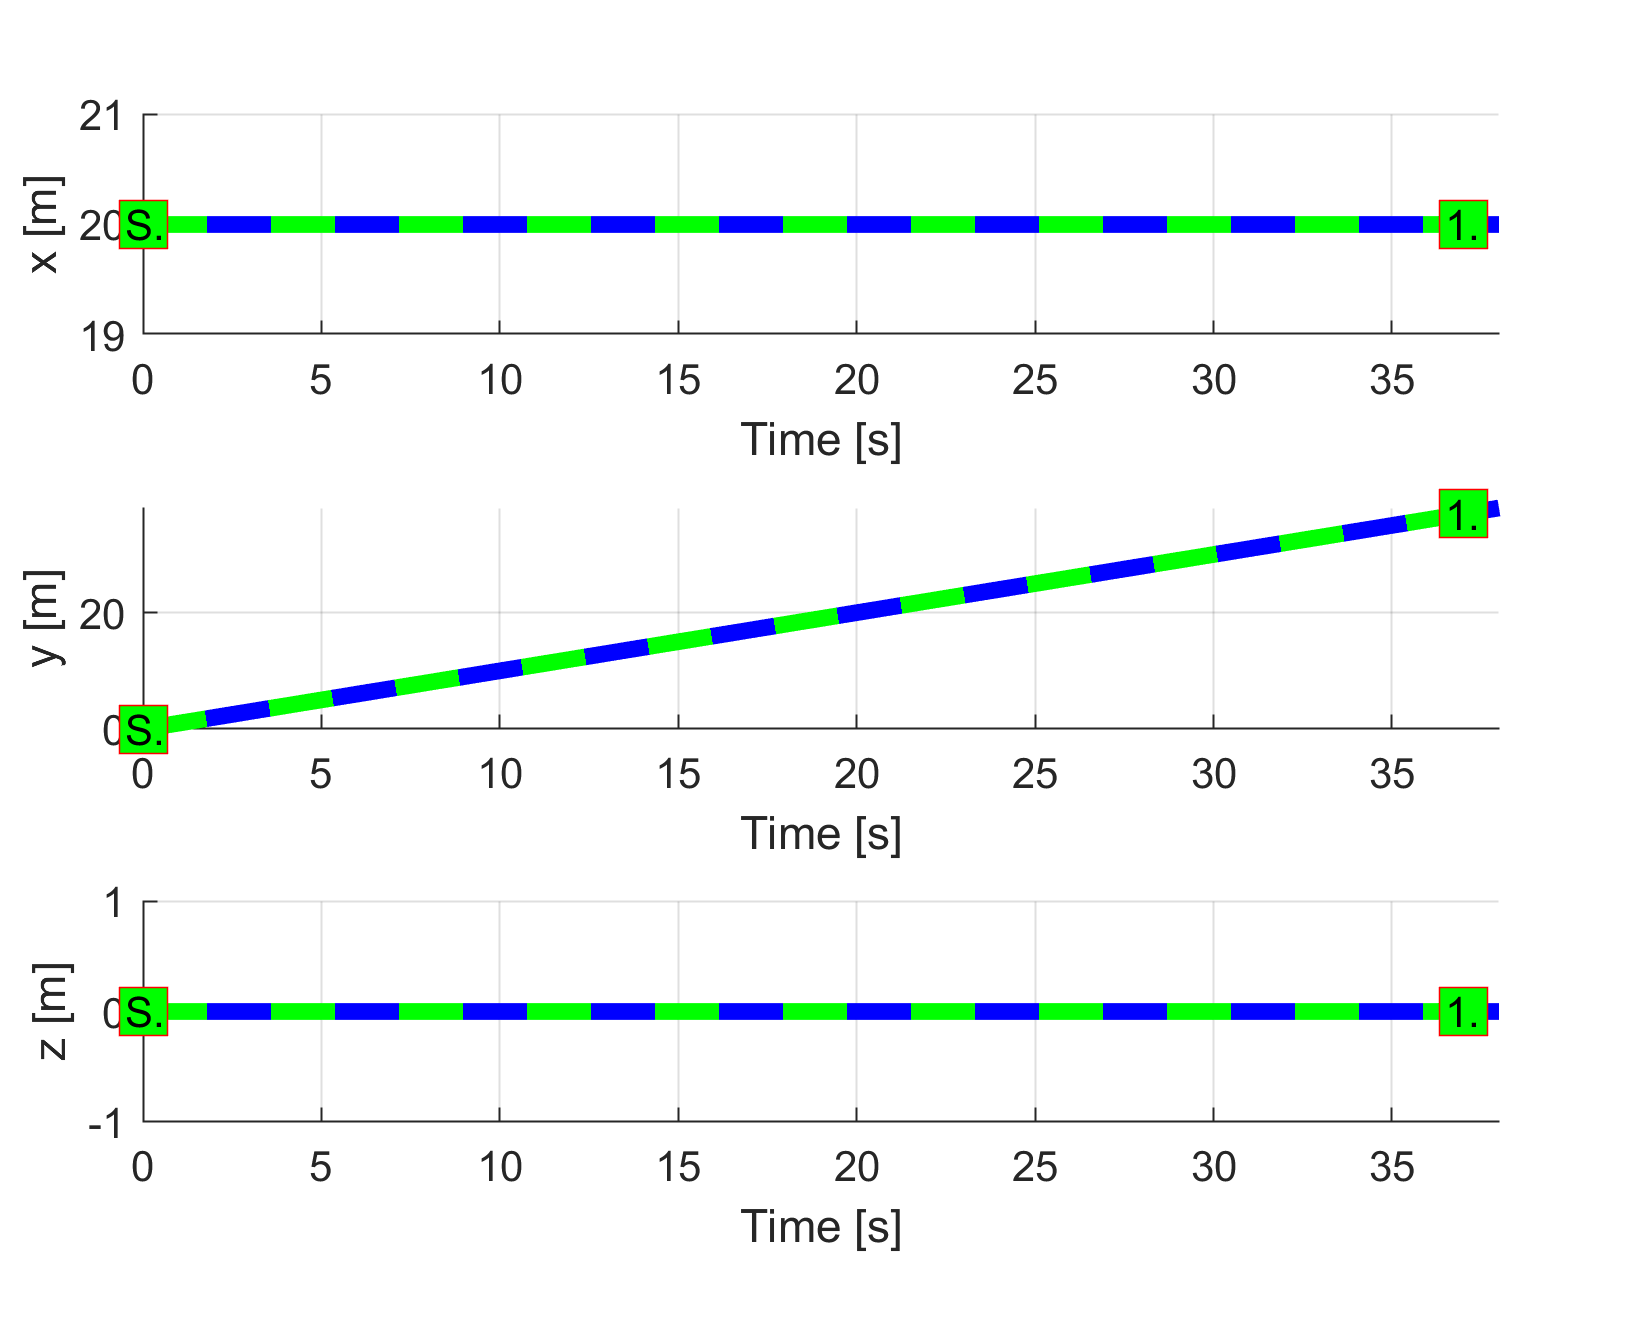
\includegraphics[width=0.9\linewidth]{\FIGDIR/NS031UtmEmergencyConvergingUAV2PathFollowing} 
        \caption{UAS 2.}
        \label{fig:emergencyCovnergingUAS2PathTracking}
    \end{subfigure}
    \caption{\emph{Trajectory tracking} for \emph{Emergency converging} test case. }
    \label{fig:emergencyConvergingTrajectoryTrackingPerformance}
\end{figure}

\paragraph{Path Following Deviations:} \emph{Deviations} (tab. \ref{tab:pathTrackingParametersForEmergencyConverging}) are in expected ranges considering the  \emph{mission plans} (tab. \ref{tab:missionSetupEmergencyConvergingScenario}) and \emph{separation safety margin} (tab. \ref{tab:aboidanceParametersForEmergencyConvergingScenario}).
    
\begin{table}[H]
    \centering
    \begin{tabular}{c||c|c}
        \multirow{2}{*}{Param.} & UAS 1     & UAS 2\\\cline{2-3}
                        & $\mathscr{WP}_1$  & $\mathscr{WP}_1$\\\hline\hline
          $\max |x|$    & 0                 & 0 \\\hline
          $\max |y|$    & 3.25              & 0 \\\hline
          $\max |z|$    & 0                 & 0 \\\hline
          $\max dist.$  & 3.25              & 0 \\
    \end{tabular}
    \caption{Path tracking properties for \emph{Emergency converging} scenario.}
    \label{tab:pathTrackingParametersForEmergencyConverging}
\end{table}


